\subsubsection{Optimal cost spanning trees}

Spanning trees are very common because they are used in a wide range of applications such as network design, IP network protocols, enterprise storage, etc.

\begin{examplebox}[: introduction to finding the best and optimal cost solution]
    Design a communication network so as to connect $n$ cities at \textbf{minimum total cost}.

    The model is made up as follows:
    \begin{itemize}
        \item Graph $G = \left(N,E\right)$ with $n = \left| N \right|$, $m = \left| E \right|$
        \item Cost function $c: E \rightarrow c_{e} \in \mathbb{R}$, with $e = \left\{u,v\right\} \in E$.
    \end{itemize}
    \begin{center}
        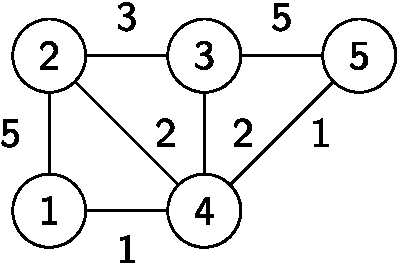
\includegraphics[width=.3\textwidth]{img/trees-6.pdf}
    \end{center}

    The required properties are:
    \begin{itemize}
        \item Each pair of cities must communicate, then the connected subgraph containing all the nodes.
        \item The minimum total cost, then the subgraph must have no cycles.
    \end{itemize}

    We give two solutions, where the second is better because it is more feasible and optimal:
    \begin{enumerate}
        \item $c\left(T_{1}\right) = 15$
        \begin{center}
            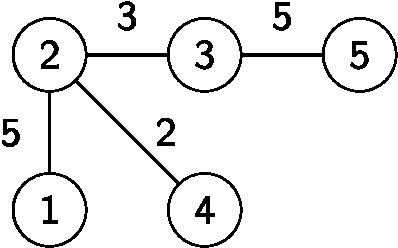
\includegraphics[width=.3\textwidth]{img/trees-7.pdf}
        \end{center}

        \item $c\left(T_{2}\right) = 6$
        \begin{center}
            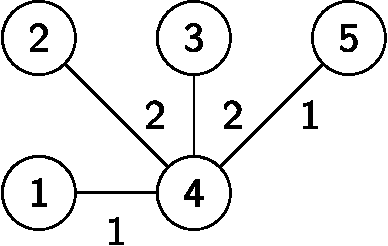
\includegraphics[width=.3\textwidth]{img/trees-8.pdf}
        \end{center}
    \end{enumerate}
\end{examplebox}

\newpage

\noindent
In general, we can formalize the \definitionWithSpecificIndex{optimal cost}{Optimal Cost} as follows. Given an undirected graph $G = \left(N,E\right)$ and a cost function, \textbf{find a spanning tree} $G_{T} = \left(N, T\right)$ \textbf{of minimum total cost}:
\begin{equation}
    \underset{T \in X}{\min} \displaystyle\sum_{e \in T} c_{e} \hspace{2em} \text{where } X \text{ is the set of all spanning trees of } G
\end{equation}

\highspace
Doesn't exists only one spanning tree, they are multiples. But the number of spanning trees available in a complete graph is defined by a theorem.
\begin{theorem}[Cayley, 1889]
    A complete graph with $n$ nodes ($n \ge 1$) has $n^{n-2}$ spanning trees.
\end{theorem}

\noindent
In general, the problem of finding a spanning tree with minimum total cost is also called \definitionWithSpecificIndex{minimum spanning tree (MST) problem}{minimum spanning tree (MST) problem}. It plays an important role in many networking applications, such as routing and networking.\cite{10.1007/978-3-642-38853-8_14}

\newpage

\paragraph{Prim's algorithm}\label{paragraph: Prim's algorithm}

\begin{definitionbox}[: Prim's]
    \definition{Prim's algorithm} is a \textbf{greedy algorithm that finds a minimum spanning tree for a weighted undirected graph}. This means it \textbf{finds a subset of the edges that forms a tree that includes every vertex, where the total weight of all the edges in the tree is minimized}. The algorithm operates by building this tree one vertex at a time, from an arbitrary starting vertex, at each step adding the cheapest possible connection from the tree to another vertex. Finally, \textbf{Prim's algorithm is exact} (it provides an optimal solution for every instance).
\end{definitionbox}

\highspace
A \definitionWithSpecificIndex{greedy algorithm}{Greedy algorithm} constructs a \textbf{feasible solution iteratively by making a \dquotes{locally optimal} choice at each step, without reconsidering previous choices}. In Prim's algorithm, at each step a minimum-cost edge is selected from those in the cut $\delta\left(S\right)$ induced by the current set of nodes $S$. Unfortunately, for most discrete optimization problems greedy-type algorithms yield a feasible solution with no guarantee of optimality.

\highspace
According to the definition of a greedy algorithm, the main idea of Prim is to build a spanning tree iteratively. It \textbf{starts with an initial tree} $\left(S,T\right)$ with $S = \left\{u\right\}$ ($u \in N$, so it can be any node in the set $N$) and $T = \emptyset$. At \textbf{each step}, \textbf{add} to the current sub-tree $\left(S,T\right)$ \textbf{a minimum cost edge} among those that connect a node in $S$ to a node in $N \setminus S$.

\begin{examplebox}[: Prim's algorithm]
    Suppose we have the following graph:
    \begin{center}
        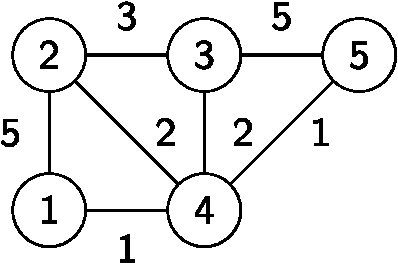
\includegraphics[width=.3\textwidth]{img/prims-alg-1.pdf}
    \end{center}

    \begin{enumerate}
        \item We start from an arbitrarily node $u$ that it is in the set $N$, for example $3$:
        \begin{center}
            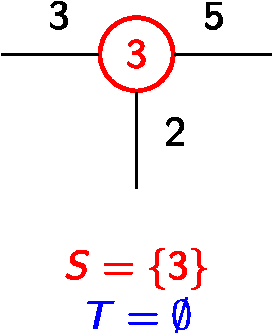
\includegraphics[width=.2\textwidth]{img/prims-alg-2.pdf}
        \end{center}

        \item As we said, at each step we add to the current subtree $\left(S, T\right)$ a minimum cost edge among those that connect a node in $S$ to a node in $N \setminus S$. So at this step we choose \emph{node 4} because the edge starting from \emph{node 3} is the less weighted edge.
        \begin{center}
            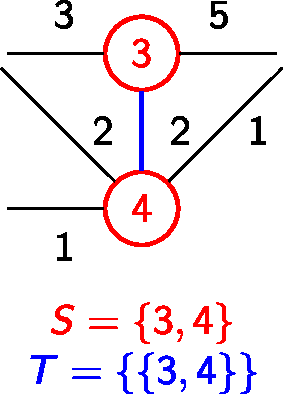
\includegraphics[width=.2\textwidth]{img/prims-alg-3.pdf}
        \end{center}

        \item At this point we continue with the same logic. The edge, starting from \emph{node 4}, with less weighted edge is \emph{node 1}. Note that at parity of the weighted edge, it doesn't matter which one we choose. Maybe the decision will lead to a different subgraph, but Prim's algorithm is greedy by definition, then it doesn't think about these problems; it assumes that it is a locally optimal choice.
        \begin{center}
            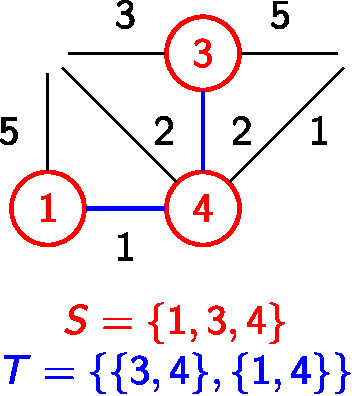
\includegraphics[width=.25\textwidth]{img/prims-alg-4.pdf}
        \end{center}

        \item Since we are lucky, the previous doubt is useless (with parity of weighted vertices, which should we choose?). Because \emph{node 1} exposes an edge with a weight of 5, but \emph{node 4} has a weighted edge of only 1, the choice is clear.
        \begin{center}
            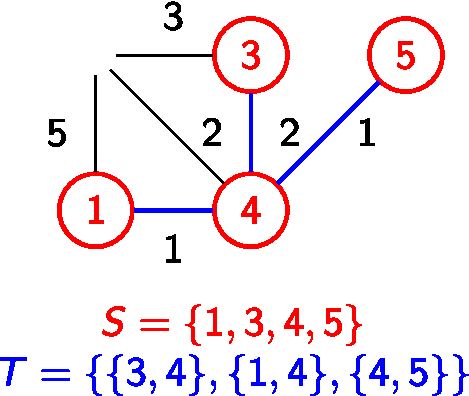
\includegraphics[width=.3\textwidth]{img/prims-alg-5.pdf}
        \end{center}

        \item Finally, we choose the edge with a weight of 2 (to the \emph{node 2}) because is the lowest. At this step, the algorithm is finished because there are no more vertices ($S = N$). The cost function returns the value $6$ (sum of each weighted edge selected).
        \begin{center}
            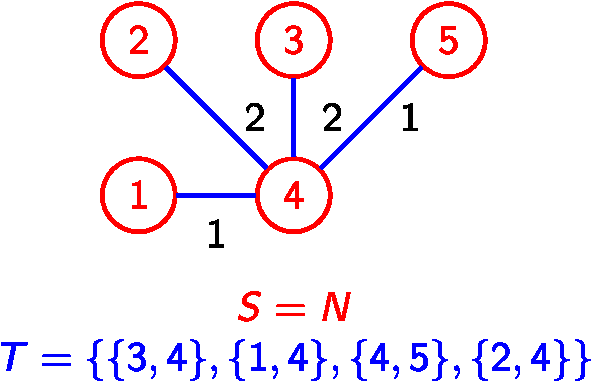
\includegraphics[width=.4\textwidth]{img/prims-alg-6.pdf}
        \end{center}
    \end{enumerate}
\end{examplebox}

\noindent
From the previous example it should be clear that at each step the Prim's algorithm creates the need to solve a minimum search problem.

\highspace
The Prim's algorithm take:
\begin{itemize}
    \item Input: a connected graph $G = \left(N,E\right)$ with edge costs.
    \item Output: a subset $T \subseteq N$ of edges of $G$ such that $G_{T} = \left(N,T\right)$ is a minimum cost spanning tree of $G$.
\end{itemize}

\begin{lstlisting}[language=pseudo-code, caption={Minimum spanning tree (MST) problem: Prim's $O\left(nm\right)$}]
S $\leftarrow$ $\{$u$\}$; $\label{prims: s-definition}$
T $\leftarrow$ $\emptyset$; $\label{prims: t-definition}$
while $\left|T\right| < n-1$ do: $\label{prims: while cycle}$
    $\left\{u\right\} \leftarrow$ edge in $\delta(S)$ of minimum cost; // with $u \in S$ and $v \in N \setminus S$ $\label{prims: search minimum}$
    $S \leftarrow S \cup \left\{v\right\}$; $\label{prims: add destination vertex}$
    $T \leftarrow T \cup \left\{\left\{u,v\right\}\right\}$ $\label{prims: add tuple source destination}$
\end{lstlisting}
\begin{itemize}
    \item[Rows \ref{prims: s-definition}-\ref{prims: t-definition}.] Declare the general sets $S$ and $T$. The first is filled with the starting node $u$ and the second is empty, because the core of the algorithm has not yet started.

    \item[Row \ref{prims: while cycle}.] Continue building the spanning tree until the length of the set of transitions $T$ is not equal to the number of nodes minus one.

    \item[Row \ref{prims: search minimum}.] Find the edge with the lowest weight from the set $\delta\left(S\right)$. Then choose one of the edges with the lowest weight and the corresponding target node. Obviously the target node $v$ cannot be already evaluated ($v \in N \setminus S$) and the source node $u$ must be in the set of nodes already evaluated ($u \in S$).
    
    \item[Rows \ref{prims: add destination vertex}-\ref{prims: add tuple source destination}.] Therefore, the most complex part of the algorithm (minimum search) is to store the target vertex with the lowest edge weight and add the tuple (source node, target node) to the set $T$.
\end{itemize}
The complexity of the algorithm is pretty much guessed. Or in the better case neither worst case, we need to evaluate each node. Then the main difference is made by the weighted edge search. If each edge has to be analyzed at each iteration, the \textbf{complexity} order is given by $O\left(nm\right)$.